% $Id$
\documentclass[a4paper,11pt, titlepage]{article}

\usepackage{a4wide}
\usepackage{hyperref}
\usepackage{listings, color, parskip,}
\usepackage{graphicx, subfigure }


\setcounter{secnumdepth}{3}
\setcounter{tocdepth}{3}

\hypersetup{
  pdftitle={Improving code documentation via smart searching},
  pdfauthor={Authors all over the place},
  pdfsubject={Improving code documentation via smart searching},
  pdfkeywords={scala, documentation, searching},
  colorlinks=true,
  linkcolor	= black
}

\lstdefinelanguage{Scala}{
  morekeywords={abstract,case,catch,class,def,
    do,else,extends,false,final,finally,
    for,if,implicit,import,match,mixin,
    new,null,object,override,package,
    private,protected,requires,return,sealed,
    super,this,throw,trait,true,try,
    type,val,var,while,with,yield},
  otherkeywords={=>,<-,<\%,<:,>:,\#,@},
  sensitive=true,
  morecomment=[l]{//},
  morecomment=[n]{/*}{*/},
  morestring=[b]",
  morestring=[b]',
  morestring=[b]"""
}

\title{\textbf{Improving code documentation\\via smart searching}}

\author{Authors all over the place\\
\\
Department of Computing\\
Imperial College London
} 
\date{\small{March 2011}}

\begin{document}
\lstset{
  language=Scala,
  captionpos=b,
  basicstyle= \sffamily ,
  breaklines=true,
  breakatwhitespace=true,
  numbers=left,
  numberstyle=\tiny,
  extendedchars=true,
  columns=fullflexible,
  tabsize=2
}

\maketitle
\thispagestyle{empty}
\tableofcontents
\newpage

\section{Introduction}\label{sec:intro}
% section intro
Exploring the documentation APIs in large codebases can be challenging. Many tools have been developed to help managing the API documentation - Javadoc for Java; Sandcastle for .NET, RDoc for Ruby . Searching functionality is essential for these tools, especially in large codebases. 

Scaladoc is a tool for generating API documentation from Scala codebases. Collaborative Scaladoc (Colladoc) is an extension of Scaladoc which enables wiki-like editing of the API documentation. Although Colladoc is a promising upgrade of Scaladoc, it lacks useful search capability.

Implementing search functionality well has many high-level challenges - usability, good search performance, providing intuitive syntax and relevant results.

The aim of the Colladoc Smart Search project is to provide efficient, easy to use smart search for Colladoc. This extension provides full-text search as well as search for identifiers, symbols and documentation comments. A goal of the project is to support a powerful query syntax that resembles the Scala language.

The document is organized as follows: Section \ref{sec:spec} discuss the status of the planned project’s requirements. Section \ref{sec:design} gives brief overview of the project architecture. Section \ref{sec:implementation} explaining our main design and implementation decisions, Section \ref{sec:methodology} presents our planning strategy and development approaches, Section \ref{sec:groupwork} presents the division of work between the team members. Section \ref{sec:finalproduct} gives an overview of the project, outlines out main challenges and achievements, provide some concrete measures about the code quality and product performance. 
\section{Specification}\label{sec:spec}
% section specification

The requirements specification identifies the target users of the Colladoc Smart Search and goes over the product use cases. The requirements, use cases and queries are prioritized in two categories:

\begin{itemize}
\item  Essential - describe functionality that is fundamental to the project and will be implemented during  the development stage.

\item  Non-Essential - describe functionality that would be beneficial to the project but is not guaranteed to be delivered.
\end{itemize}

\subsection{Target Users}

[u1] Developer - a person with working knowledge in Scala. Sometimes he searches for packages, classes, objects etc. The developer searches for something specific.

[u2] Technical Writer - a person responsible for writing documentation. He needs a quick 
overview of missing or updated documentation. He needs to limit searches to the packages and classes that he is working on.

[u3] Beginner - a person learning the Scala language or starting on a Scala-based project. He may not be familiar with Scala syntax and needs helpful search results from general queries.

\subsection{Functional Requirements}

\subsubsection{Essential Functional Requirements}
\indent [c1] When the user enters a search query, the search results page should displays all entities that match the query. 
We have implemented all essential queries that were planned \emph{\color{red}see example queries}.

[c2] When the user is on the search results page, clicking on the entity name (1) toggles its details (2).
We have implemented this functionality.

\begin{figure}[h!t]
\begin{center}
\leavevmode
\fbox{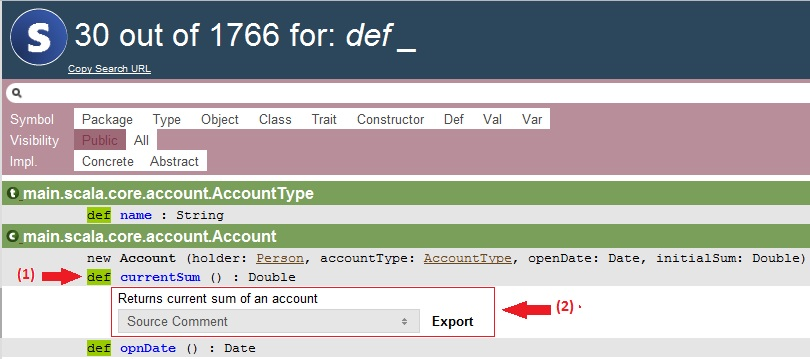
\includegraphics[width=0.9\textwidth]{c2}}
\end{center}
\caption{Toggle User Details}
\label{fig:toggle_user_details}
\end{figure}


[c3] When the user does not enter anything, search is not triggered.
We have implemented this functionality.

[c4] The search result page support filtering of the results. Filtering can be done either by entity type using predefined filters (2) or by entity name (1) . 
We have implemented this functionality.
\begin{figure}[h!t]
\begin{center}
\leavevmode
\fbox{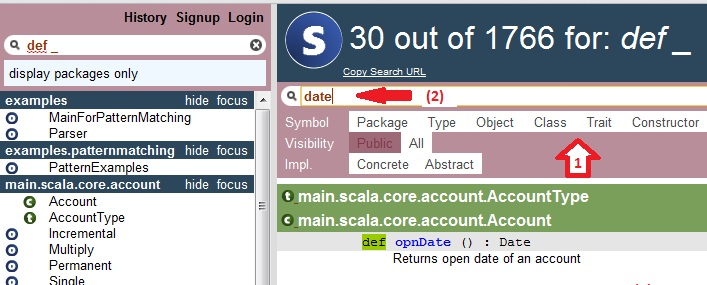
\includegraphics[width=0.9\textwidth]{c4}}
\end{center}
\caption{Filter Results}
\label{fig:filter_results}
\end{figure}

[c5] When entity comment is updated, searching the changed documentation should contain the updated entities.
We have implemented this functionality.

\textbf{Essential Query Examples}

Table~\ref{essential_query_examples} contains examples of the essential query language constructs. 
\begin{table}[htbp]
\begin{center}
\begin{tabular}{|p{1.4in}|p{0.7in}|p{1.8in}|p{0.4in}|} \hline 
\textbf{User Query/Search} & \textbf{Syntax} & \textbf{Results Produced} & Status  \\ \hline 
[q1] Any text ``Foo''. & Foo & - Comments that contain text ``Foo''\newline - All entities (types/packages/methods) with names containing the text Fooe.g. class FooBar, trait MyFooTrait & done \\ \hline 
[q2] Text ``Foo'' exactly. & ``Foo'' & - Comments that contain ``Foo'' exactly\newline - Entities named exactly ``Foo'' & done \\ \hline 
[q3] Text ``Foo'' in comments. & // Foo & Comments that contain text ``Foo''. & done \\ \hline 
[q4] Classes\textbackslash objects\textbackslash \textbf{ }
traits\textbackslash packages named ``Foo''. & class Foo; object Foo; trait Foo; package Foo & Entities named ``Foo'' exactly. & done \\ \hline 
[q5] Classes\textbackslash objects\textbackslash \textbf{ } traits\textbackslash packages whose names end with ``Foo'' & class \_Foo; object \_Footrait \_Foo; package \_Foo & Entities with names ending with ``Foo''.\newline e.g. Foo, MyFoo & done \\ \hline 
[q6] Classes that extend class ``BaseFoo'' & extends BaseFoo & All classes that derive from ``BaseFoo''.\newline e.g. DerivedFoo & done \\ \hline 
[q7] Classes that implement trait ``FooTrait'' & with FooTrait & All classes that implement the trait ``FooTrait''. & done \\ \hline 
[q8] Methods named ``bar'' & def bar & All methods (any number of parameters and any return type) that are named ``bar'' & done \\ \hline 
[q9] Methods that return Int & def \_ : Int & All methods that return Int & done \\ \hline 
[q10] Methods that have two parameters, an Int and a String, and return Int & def \_(Int, String): Int & All methods that take an Int and a String and return Int. e.g. bar(i: Int, s: String) : Int\newline \newline This will also return equivalent curried functions e.g. bar(Int)(String) & done \\ \hline 
[q11] Method that takes an Int parameter, followed by zero or more parameters & def \_(Int, *) & All methods that take an Int and zero or more parameters & done \\ \hline 
[q12]  Values or variables called ``name'' & val name:String\newline var name:String & All member values or variables that are named ``name'' and are of type String. The results are ordered by val / var depending on the query. & partial \\ \hline 
\end{tabular}
\caption{Essential Query Examples}
\label{essential_query_examples}
\end{center}
\end{table}

\subsubsection{Non Essential Functional Requirements} 
\indent \indent [c6] Technical Writer searches for the entities in a package. Then he filters the results to entities with no documentation by selecting an option on the page. We have not implemented this requirement due to time constraints, but the system can be easily extended to support it.

[c7] The user searches for the entities in a package. If no result is found, a help page is displayed. The help page contains sample queries that (1) as well as option for searching that query input in Google (2).
We have implemented this functionality. Additionally, we have provided a Syntax Reference page that provides query examples for the supported syntax.

\begin{figure}[h!t]
\begin{center}
\leavevmode
\fbox{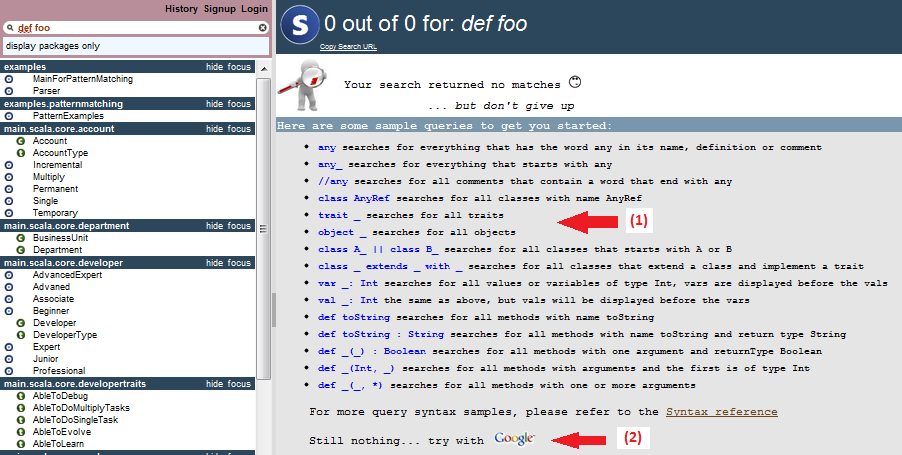
\includegraphics[width=0.9\textwidth]{c7}}
\end{center}
\caption{Filter Results}
\label{fig:filter_results}
\end{figure}

[c8] The user searches for an entity. If there is only one search match, the result will be the documentation page of the given entity.
We have not implemented this requirement due to time constraints.

[c9] The user browses the search results. He wants to see only one type of entity. He chooses this by clicking an option in the results filter. 
We have implemented this functionality.

[c10] The Developer wants to see where a class is used in the API. He searches for the exact name of the class. The search returns all the API visible usages of the class. As a result of discussion with our supervisors, we decided that this requirement does not provide any benefits to the current project and is not related to our final goal. Therefore, this functionality was not implemented.

[c11] A user searches for the entities in a package. Then he filters the results to entities that contain code snippets in their comments.
After discussion with our supervisors, we set low priority for this requirement. We do not see this feature providing great benefit to the user. There are better ways to look for code snippets: blogs, articles and so on. Moreover,  we could not find any example of code in the comments of the codebases we looked at. We have not implemented this functionality.

We have managed to extend the query syntax so it supports most of the initially specified non-essential queries. 

The syntax that is not currently supported is [q13] and [q20]. [q13] was not implemented because of the large development effort required. Additionally, omitting this query does not limit what the user can search for. [q20] was not implemented due to time constraints. 

We recognised that our initial query syntax specifications did not support some important queries. We realised that if we omitted these queries, it would restrict the users ability to search for some language constructs. Therefore, we have added two more search features to the syntax: search for tuples [q21] and search for entities with reserved names [q22]. This is supported by the language and is commonly used in many Scala libraries. 

Additionally, we changed the syntax of query [q18] in order to comply with the Scala syntax. Also [q12] is partially imported - the syntax is supported, but due to time constraint we have not implemented ordering based on whether the user search for val or var.

\textbf{Non-Essential Query Examples}

Table~\ref{non_essential_query_examples} contains examples of the essential query language constructs. 
\begin{table}[htbp]
\begin{center}
\begin{tabular}{|p{1.4in}|p{1.2in}|p{1.3in}|p{0.5in}|} \hline 
\textbf{  User Query/Search Syntax}\newline \textbf{} & \textbf{Syntax } & \textbf{Results Produced} & \textbf{Status} \\ \hline 
[q13] Search using logical AND. e.g. search for classes named ``Foo'' and classes that contain a method ``bar''. & class Foo AND def barclass Foo \&\& def bar & All classes named Foo that contain a method bar & not done \\ \hline 
[q14] Search using logical OR.\newline e.g. search for methods named ``add'' or methods named ``sub'' & def add OR def sub\newline def add \textbar \textbar  def sub & All methods named ``add'' or methods named ``sub''. & done \\ \hline 
[q15] Search using the NOT operator. e.g. search for classes that end with text ``Foo'', but exclude classes named ``BaseFoo'' from the results & class \_Foo not class BaseFoo\newline class \_Foo !class BaseFoo & All classes that end with ``Foo'' but not class ``BaseFoo'' & done \\ \hline 
[q16] Search using query grouping. e.g. search for classes named ``Bar'' or for classes with names ending in ``Foo'' but not ``BaseFoo'' & class Bar OR (class \_Foo NOT class BaseFoo) & All classes named Bar in addition to classes that end with ``Foo'' but not class ``BaseFoo'' & done \\ \hline 
[q17] Search for method that takes a function as a parameter. & def \_(Int =$>$ String) & All methods that take one parameter which is a function with signature Int =$>$ String & done \\ \hline 
[q18] Search for all methods with two parameters, an Int and a String, and return Int & Int =$>$ String =$>$ Int\newline (Int, String) =$>$ Int & All methods that take an Int and a String and return Int.\newline e.g. bar(i: Int, s: String) : Int & modified \\ \hline 
[q19] Search for a generic class with one parameter & class \_[A] & All classes with one generic parameter & done \\ \hline 
[q20] Search for a generic method called ``foo'' with two generic parameters. & def foo[A,B](A, B, Int) & Returns all methods called foo with two generic parameters and the respective argument types. & not done \\ \hline 
[q21] Search for Tuples & def \_:(A,B) & Returns all methods that return a two-element tuple with of types A and B & done\newline (new) \\ \hline 
[q22] Search for keywords & def `def` & Returns all methods named ``def'' & done\newline (new) \\ \hline 
\end{tabular}
\caption{Non-Essential Query Examples}
\label{non_essential_query_examples}
\end{center}
\end{table}

\subsection{Non-Functional Requirements}

\subsubsection{Essential Non-Functional Requirements}


[n1] The search results should appear in less than 5 seconds. 
We have achieved this requirement. With the largest codebase we have tried, the results appeared in less than two seconds. For more details, see Final Product - Performance section.

[n2] The source code of Colladoc Smart Search will contain unit tests for most of the newly added classes.
We have achieved \emph{\color{red}92} \% code coverage.For more details, see \emph{\color{red} Final Product - Testing}.
[n3]The source code will follow the coding style and formatting of the existing Colladoc code.
This requirement has been achieved. We have created Coding Style document \cite{coding-style} and have adhered to it throughout development. 

\subsubsection{Non Essential Non-Functional Requirements}

[n4] End-to-end integration tests for the essential search functionality will be created.
This requirement has been achieved. For more details, see Final Product - Testing.
[n5] The results should be displayed immediately in the results page. The user should not wait for all of the results to be fetched if they are more than 5 entities.
This requirement has been achieved. \emph{\color{red} See Design- Infinite scrolling section}

\section{Design}\label{sec:design}
% section outcomes
This section provides the overall architecture of our project and discusses the main design choices that we made.

An understanding of the existing Colladoc architecture was necessary to ensure that the system implemented would fit seamlessly into the existing product. 
Many of the design decisions that we made were influenced by the fact that Colladoc Smart Search is an extension to Colladoc.
Fig. \ref{fig:product-design} shows the original Colladoc architecture in italic and Colladoc Smart Search extensions in bold. 
\begin{figure}[h!t]
\begin{center}
\leavevmode
{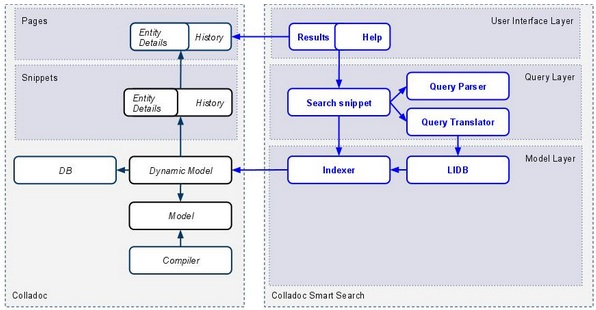
\includegraphics[width=0.9\textwidth]{design}}
\end{center}
\caption{Product Design}
\label{fig:product-design}
\end{figure}
Colladoc uses the Scala compiler front-end to create a documentation model (or just Model) from the source code input. This documentation model is used to provide the symbol information and code documentation that is visualised in Colladoc. Wiki-like editing of documentation is achieved by extending the original model to a Dynamic Model, which allows documentation changes. Changes for each documentation symbol are persisted in a database. “Snippets”
generate dynamic content based on the information provided by the Model. Pages visualize this content.

The overall design of Colladoc Smart Search separates the system into layers. We defined three layers of Colladoc Smart Search  - Model, Query and UI layers. 

The \textbf{Model layer} contains components which access the documentation model, analyze it and add it to a search index database. ${SearchIndexer}$ is the main component in that layer.

The \textbf{Query layer} contains components which take search queries,  execute them and return the result. When the user enters a search query string, the $SearchSnippet$ passes it to a $QueryParser$ that generates an abstract representation of the query. The search-engine independent representation is transformed by Query Transformer to specific query objects used by the search engine. The $SearchSnippet$ generates the search result content and passes it to the UI layer.

The \textbf{UI layer} contains components which present the search results to the user.
\section{Implementation}\label{sec:implementation}
% section conclusion
This section contains the Colladoc Smart Search implementation details. We outline the main implementation choices and explain the reasons for them. 

The original Colladoc uses Lift 2.0 as for web application framework. In extending Colladoc, we followed that. Colladoc uses a MVVM pattern \cite{lift} \emph{\color{red} why the star is here?}, which means that the application is split into a Model - View - ViewModel which map closely to our Model - UI - Query layers respectively.

The MVVM pattern is classic three-layer application pattern similar to MVC and MVP. In the MVVM pattern the Model contains data; the ViewModel contains the business logic. It also matches the View closely in structure and handles events coming from the View; The View visualises the ViewModel.
\begin{figure}[h!t]
\begin{center}
\leavevmode
{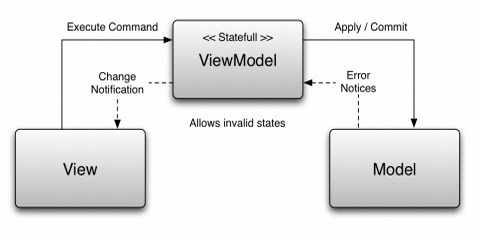
\includegraphics[width=0.9\textwidth]{mvvm}}
\end{center}
\caption{MVVM as explained in \cite{lift}}
\label{fig:mvvm}
\end{figure}

\subsection*{Model Layer}
For the data indexing we used Apache Lucene, an open source search engine. Our team member – Rumyana Neykova – had prior experience with it and Lucene was the suggested indexing technology in the initial project proposal, so we did not consider any other search engines.

\textbf{When we index}\\ 
The indexing is done by the $SearchIndexer$ class. We agreed on synchronously indexing the entire documentation model right after it is constructed (i.e. when the application is launched) to eliminate the overhead when performing searches. Although we considered other indexing strategies such as waiting for the first query to index or indexing the documentation model asynchronously, those were rejected because in the first case the delay would be noticeable by the user and in the second queries executed before indexing completed would have produced incomplete results. The documentation model does not change often, so indexing upfront is justified.

The only time when the search index needs to be updated is when a user edits the documentation. Therefore, the $SearchIndexer$ has the ability to re-index individual symbols. We  obtained acceptable  performance by making the reindexing right after the user saves an edit to the documentation.

\textbf{What do we index}\\
The documentation model is indexed and stored with the help of the Lucene search engine. 
Lucene stores its contents in separate units called ‘documents’. Each document has searchable text contents. Documents are returned as a result of querying the Lucene database. The structure of the document that we stored was very important since it affects what search queries we can make and what results are returned. Therefore, we had to decide whether to have one document per class or one document per class member. Two of us (Miroslav Paskov and Jamil Rzaev) worked on the functionality in parallel for a week. It showed that storing separate documents gives us more granular results and makes the individual documents simpler, without any performance overhead. From development and maintenance perspective this was a better choice and we decided to have a more granular indexing. This decision meant that we needed to match each class member to its respective class. Lucene does not support document relations by default so we did this by assigning a unique id to each entity of the documentation model and its respective Lucene document. 

\textbf{Lucene 3.0 or Lucene 4.0}\\
Initially, we started using Lucene 3.0 as it is the latest released version of Lucene. After the project was underway we realized that the coming version of Lucene, 4.0, is a better candidate for our purpose since it allowed more precise queries to be made. Unlike Lucene 3.0, the new version does not suffer from performance drawbacks with wild-card queries (e.g. [q5], [q11]) which we expect to be often used in searches. For one week, two of us (Miroslav Paskov and Jamil Rzaev) did parallel development in both Lucene 3.0 and 4.0 to make sure that we meet the iteration’s objectives and to mitigate any potential transition problems. This was duplication of efforts but in the end we could make an objective decision to adopt Lucene 4.0.

\subsection*{Query Layer}

The $SearchSnippet$ maps to the ViewModel in the Lift MVVM pattern.

When the user enters a search query it is parsed by the $QueryParser$ class to an abstract syntax tree (AST) of the search query ($SearchQuery$ class and its descendants). This AST is search-engine independent and contains all information for the search query. It is transformed to a Lucene-specific query object (an instance of Query).

\textbf{Query Parsing or Direct Transformation} 
Simple wildcard queries (containing * or ?) can be directly transformed to a syntax that is supported by the Lucene search engine. In our initial discussion we were aiming for this approach. Early on, we agreed that we need to support complex syntax, for example:

\begin{lstlisting}
(List[_], _Map, *) => (Int, String)
\end{lstlisting}

We needed to distinguish language features such as generics, lambda parameters and tuples. This required a parser that can handle this syntax and give us more flexibility. We looked into several options for a parsing, in the first weeks of development. 

\textbf{Custom, Generated or Combinatorial Parser}\\
We started with an ad-hoc implementation of a parser. After one week it could distinguish the first three basic queries but it looked like continuing in the same style will prove to be increasingly difficult to develop and maintain. We were aware of parser generators like ANTLR or JavaCC but we expected that Scala, being partly functional, may have a language feature or library that helps parsing. We came across Combinatorial Parsers – which are a built-in library that allows defining parsers succinctly, very much like a BNF(*) grammar, for example:

\begin{lstlisting}
def expr = or | and  | term
def `val` = "val" ~> identifier ~ returnType
\end{lstlisting}
We were very happy with the clarity and expressiveness of the library and we chose it for the parser.

\textbf{How Results are Ordered}\\ 
The default ordering implemented by Lucene is used. Lucene uses result weights to determine which results come first. Result weights are calculated based on how often a word occurs in the document or whether queried terms are near each other. Only searching for text in comments produces varying result weights - this is due to how we index the documents. All other searches produce results with equal relevance.
UI Layer 

The $SearchPage$ maps to the View in the Lift MVVM pattern. Views are combination of dynamic inline HTML that renders the information in browsers. 

\textbf{Reusing Scaladoc and Colladoc UI Templates}\\
Initially we did not know how much of the existing UI code could be reused but we started work on the UI with the intention of reusing as much as possible. Thus we preserved much of the look-and-feel of Scaladoc in our results page. We reused templates for page headers, displaying results and filtering results. 

\textbf{Inline Html}\\
As a rule, we followed the existing coding style. Our UI code contains inline HTML literals which may not be a good coding practice but it made our new code consistent with existing code. We decided it was more important to follow the existing coding style for maintainability and not introduce a new one.

\textbf{Infinite Scrolling (Lazy loading) or Pagination}\\
Infinite scrolling is a UI pattern where only a part of a longer content will be initially loaded. When the user scrolls down to reveal more content, it gets asynchronously loaded. Initially, we decided to implement pagination for longer search results then we agreed that infinite scrolling gives better user experience. It allows the user to continue to view content on a single page without having to leave it. No clicks are needed to load more information on the page.

\textbf{Implementing Infinite Scrolling}\\
We had the option to either use an existing infinite scrolling library or implement it ourselves. It turned out that existing libraries did not fit very well with our current implementation and it would be easier to implement it ad-hoc.

The infinite scrolling has two major elements:
\begin{enumerate}
\item The Lucene IterablePagingCollector class which only reads a subset of all results for a query.
\item A jQuery script - that listens for when the page is scrolled to the bottom and makes an AJAX call for the continuation of the results, depending on how many results have been retrieved so far.
\end{enumerate}

\section{Methodology}\label{sec:methodology}
% section outcomes

This section describes the methodologies and techniques we have used to complete the various tasks and challenges we encountered throughout the project.

{Planning}

Strategically planning the division of the overall task into manageable sub-problems was essential to the project’s success. Our overall strategy for the project was to achieve a working product with the core functionality required as early as possible and then to focus on implementing features that enhance this core functionality.

One technique that we found very useful was brainstorming - it helped to bring out all ideas that we individually had about the project and to structure and reconcile them. We did brainstorming about the project scope and specification; its use cases and the contents of the three projects reports.

We decided to divide the tasks based on the architecture layer that they belonged to. We set one task per day for each team member, the task was small enough to be completed in that time. We balanced the project tasks with other assignments that each team member had. We initially focused on the Model Layer tasks, extending to Query and UI Layers later. After the first few weeks we worked on all layers in parallel. 

\emph{\color{red}For more details about the project plan} refer to the Logbook in the Appendix.

\subsection{Development Approach}

Throughout the course of the project we used an iterative development approach. More specifically, we incorporated key practices from agile development, such as iterations, scrum meetings and pair programming and tailored them to suit our needs.

Our work was done in a series of iterations (two iterations per week). At the start of every iteration, we had a retrospective discussion on each of the work items from the previous iteration and then planned the work that each team member would do during the next iteration. We had a detailed project schedule which included the daily tasks and progress of each team member. The Logbook in the Appendix is based on it. 

The team met at least once during each iteration to work together on the tasks that were assigned. In order to improve the development process further, we set automatic mail notification with each code check-in.

At the end of every two iterations, we gave a product demonstration to our supervisors to show the progress that had been made during the week. The team found this approach to be very efficient since it structured our schedule in a way that ensured regular team meetings and continuous communication. Getting feedback early on prevented us from wasting time implementing inessential requirements and allowed us to extend the product with new useful functionalities. Keeping minutes for each of our meetings helped us to log and act on all feedback. Scheduling regular demonstrations also helped the team to focus on having an iteratively fully working product throughout the development. Additionally, we have found that this iterative style of development helped us to split our overall project goal into a series of manageable sub-tasks and sub-goals.

In addition to iterations, the team also defined a set of three product milestones, which are specific dates where we expected the project to have a certain set of features. These higher-level divisions in the project schedule were very helpful in setting a specific context for the planning of iterations. 

\subsection{Quality Assurance}

Setting up the testing infrastructure was one of our first tasks. We have different types of tests for our product:
\begin{itemize}
\item Query Parser Unit Tests – The tests are written in Scala using JUnit.
\item Model Unit Tests – We used Scala Specs, JUnit and JMock. Specs is a library that allows expressing unit tests more naturally. We used JMock to isolate our tests from the real model objects generated by the Scala compiler. The tests check that the given model (package, class, member, etc) is correctly stored in the Lucene index.
\item Integration UI Tests. One of our first tasks was to create a proof-of-concept UI test using the Selenium IDE and integrate the test into our codebase. The UI is the only part of the system that has no individual unit tests but we believe that integration tests combined with unit tests for the Model and Query gave us confidence in our work. The Integration tests can be run from the project build tool.
\end{itemize}

A demo / test project was created that serves as test data for the Integration tests. Its contents are meant to include a variety of cases – deep class hierarchies, methods with similar signatures, similarly named types, different types of comments (class, member, parameter, return type, code example comments). Both positive and negative tests can be created without searching for a particular structure or arrangement in a real project. The demo project is updated when new test cases are identified.

There were no tests for the original Colladoc, but we decided not to test the original individually because our Integration tests cover the interaction points between our extension and the original. Furthermore, we only made minimal changes to the original Colladoc code.

We used code coverage metrics, generated by the Scala Code Coverage Tool (SCCT), to evaluate the depth of coverage that our tests provided. This helped us to identify where additional tests were needed.

We ran the Colladoc Smart Search on the largest Scala codebases we could find (Lift Web Framework and the Scala Library) during the second milestone and this helped ensure that our system scaled well to larger codebases.
\subsection{Overcoming Challenges}

We were able to overcome the intellectual and technical problems we faced during the project. Although the learning curve for the project language - Scala and the project related tools was quite steep, we organized regular presentations on what we have learned so far. This involved all team members and sped up the learning process. 
We faced several challenges during the project (initial project configuration, running the project on large code base), by persevering and working together.

We were also able to identify and mitigate high-risk project requirements and tasks so that the schedule was not jeopardised. In particular, some of the more complex query syntax ([q15]) that was specified was clearly high-risk due to the amount of work required in both the model layer and the query layer to support it. The team mitigated the risk posed by high-risk features by prioritizing the features we would implement first. More specifically, we implemented complex features and query syntax that were essential requirements (q[1] - q[5])  early on in development so that we would have a more accurate estimate of the amount of work required and could plan accordingly. In contrast, complex features and query syntax that were non-essential requirements were scheduled later in development so that they did not delay work on any essential requirements.

Another risk was how well the indexing and search would scale to large codebases. To mitigate them we ran performance investigations as early as possible.

The design decision to take a dependency on Lucene 4.0 instead of Lucene 3.0 was another high-risk task that we managed by scheduling work that we could fall-back on in case we found that Lucene 4.0 integration was not feasible. (For more details, refer to Implementation - Lucene 3.0 or 4.0)

\section{Group Work}\label{sec:groupwork}
% section Group Work
This section describes the division of work. The initial stage of the development process was  devoted to learning the Scala language and studying the code of the original system. For optimal productivity each team member focused on one or two sections of the system. We divided the work so that dependencies between team members’ tasks were minimal which is a key point of parallel development. 

\textbf{Who did what} \\
\textbf{Model} - Design; study of existing documentation model; Apache Lucene indexing; ways to index comments; asynchronous queries; demo project implementation; pagination - Everyone \\
\textbf{Query} - query syntax samples; Lucene queries; query parser; query translator - Rumyana Neykova, Jamil Rzayev, Miroslav Paskov, Akil Burgess \\
\textbf{UI} - reusable components; Lift framework; Ajax and jQuery; results page; result filters; result highlighting; permalink urls; infinite scrolling - Alakbar Ayyubov, Akil Burgess \\
\textbf{Report writing} - Everyone \\
\textbf{Testing} - Everyone.

\emph{\color{red} For more information about tasks, see the logbook in Appendix.}
\section{Final Product}\label{sec:finalproduct}
% section conclusion
Colladoc Smart Search enables users of Colladoc to explore code documentation with a powerful, intuitive search syntax. Relevant search results are presented quickly, in a way that is consistent with the Colladoc UI. This section evaluates the project’s achievements, presents evidence of quality and outlines further project extensions.
\subsection{Achievements}

\subsubsection{Achieved Project Specifications}
We achieved all essential project requirements and the majority of the non-essential ones. 
For details see Section \ref{sec:spec}.

\subsubsection{Implemented Additional Features}

We have also gone above and beyond the specifications and implemented several additional features that significantly improve user experience:

\textbf{Results Highlighting} (Fig.~\ref{fig:highlighting}) - provides the user with visual highlights of the terms in the results that match with the search query. It makes it easier for the user to find the most relevant content.

\begin{figure}[h!t]
\begin{center}
\leavevmode
\fbox{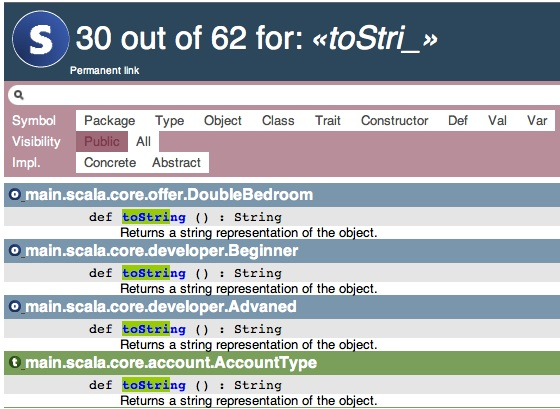
\includegraphics[width=0.7\textwidth]{highlighting}}
\end{center}
\caption{Highlighting Feature}
\label{fig:highlighting}
\end{figure}

\textbf{Infinite Scrolling} (Fig.\ref{fig:infinityscrolling})- allows the user to continuously scroll through search results without having navigate between pages.


\begin{figure}[h!t]
\begin{center}
\leavevmode
\fbox{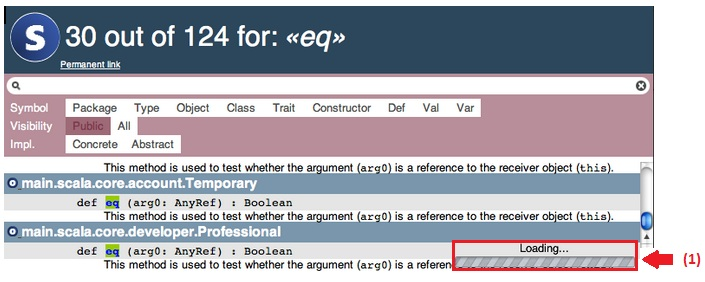
\includegraphics[width=0.7\textwidth]{infinityscrolling}}
\end{center}
\caption{Infinite scrolling feature. The loading image (1) appears to notify the user that more results are being fetched.}
\label{fig:infinityscrolling}
\end{figure}

\textbf{Other nice-to-have features} 
We added some handy shortcuts to help users navigate to the main search box. We integrated google search to help the user search in Google if his query produces no results. 

\subsubsection{Intuitive Query Syntax}
Colladoc Smart Search supports Scala-like search syntax for queries, which makes searching natural for any Scala developer. We allow searching for advanced language constructs such as currying, lambda expressions, generic classes and parameters. Additionally, support for query grouping, boolean operators and wildcards allows users to perform searches using familiar constructs from popular search engines.   
Testing

The Colladoc Smart Search project includes a variety of tests that provide comprehensive test coverage of the new functionality added and of the integration points between this new functionality and the original product.

We have added 211 new tests to Colladoc. Metrics show that our tests achieve 92\% code coverage of the new components that we added (Fig.~\ref{fig:codecoverage}). In addition, our tests achieve 56\% code coverage for the entire Colladoc codebase, which previously had no test coverage.

\begin{figure}[h!t]
\begin{center}
\leavevmode
\subfigure[Colladoc Smart Search Code]{\label{fig:codecoverage-a}
\fbox{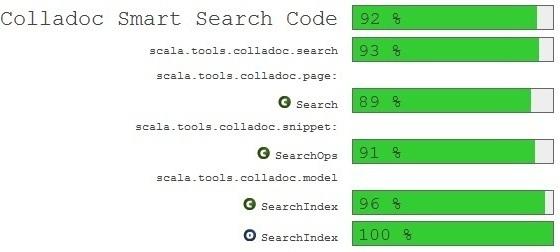
\includegraphics[width=0.4\textwidth]{codecoverage_smartsearch}}}
\subfigure[Colladoc Total]{\label{fig:codecoverage-b}
\fbox{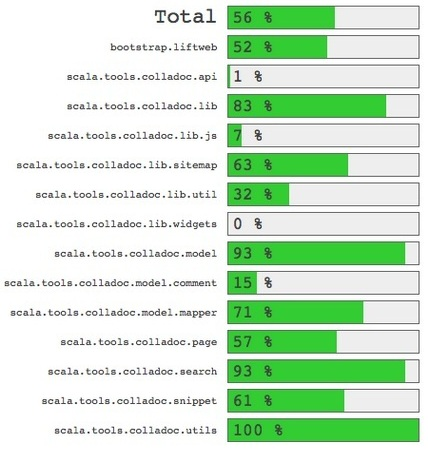
\includegraphics[width=0.4\textwidth]{codecoverage_total}}}
\end{center}
\caption{Code Coverage Results. The results are generated using SCCT}
\label{fig:codecoverage}
\end{figure}

\subsection{Performance}
We thoroughly tested Colladoc performance using several two large code bases-Lift Web Framework and Scala Library. We also use several small projects (see Table \ref{tab:test-projects})

\begin{table}
\begin{tabular}{|p{0.9in}|p{2.2in}|p{1.2in}|} \hline 
Code Base & Entities for indexing & Indexing (ms)\\ \hline 
Scala Library & 85 495\newline ( 572 scala files containing approximately 50 packages, over 1000 classes, objects and traits ) & 190 000 \\ \hline 
Lift-total & 85 902\newline (300 scala files, containing approximately 59 packages, over 1500 classes, objects and traits) &  \\ \hline 
Lift-base & 38 379 & 41709\\ \hline
Lift-modules & 18 747 & 20132\\ \hline
Lift-json &	2232 & 4370\\ \hline
Demo-Project &	1873 & 3863\\ \hline
\end{tabular}
\caption{Test Projects}
\label{tab:test-projects}
\end{table}

\textbf{Indexing performance}\\
Indexing of the documentation model for the Scala Standard Library codebase finishes in approximately 190 seconds on the Imperial College DoC lab machines. Since indexing is done only when the web application is launched, this performance is acceptable.

Fig.~\ref{fig:indexing-performance}  shows the results of indexing performance on documentation models of varying size. These results clearly show that our indexing algorithm scales well with the size of the documentation model being indexed. The linear growth in indexing time is evidence that the complexity of our indexing algorithm is ϴ(n).

\begin{figure}[h!t]
\begin{center}
\leavevmode
\fbox{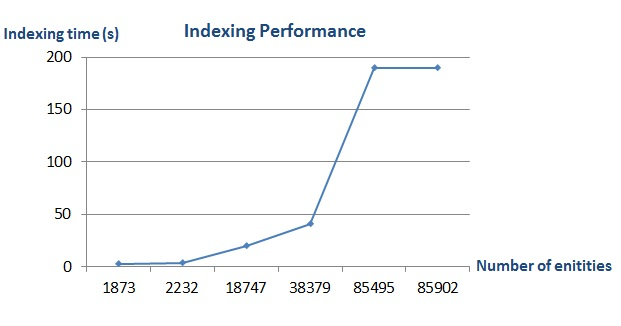
\includegraphics[width=0.9\textwidth]{indexing-performance}}
\end{center}
\caption{Search Performance}
\label{fig:indexing-performance}
\end{figure}

\textbf{Search performance}\\
Search performance on these large source codebases is very good, even for search queries that return up to 80,000 total results. Stop-watch search performance tests using several different machine configurations \emph{\color{red}(give some example machine specs here?)}, show that the first set of search results are presented to the user in less than two seconds on average. Figure \ref{fig:search-performance} depicts programmatic measurements of the time taken execute a query for different numbers of total search results. This graph shows that the time taken to execute a search is not related to total number results since we have logic to only actually fetch indexed documents for the first "page" of results. Furthermore, this highlights the fact that the product provides consistent search throughput regardless of the total number of results for a query.


\begin{figure}[h!t]
\begin{center}
\leavevmode
\fbox{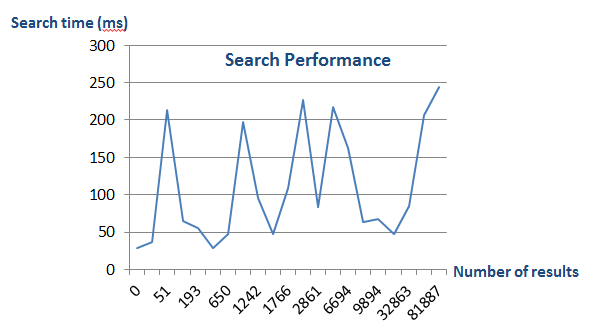
\includegraphics[width=0.9\textwidth]{search-performance}}
\end{center}
\caption{Search Performance}
\label{fig:search-performance}
\end{figure}


Performance testing clearly shows that Colladoc Smart Search provides acceptable performance for our user scenarios. Additionally, the performance of non-Smart Search Colladoc scenarios have not been degraded.

\section*{Appendix}
\addcontentsline{toc}{section}{Appendix}
\appendix
\section{Logbook}\label{sec:logbook}
This section provides information about the tasks of each team member for each iteration in the project. 

\textbf{Iteration 1, 28 Feb - 30 Jan}
Miroslav Paskov - Project Planning; Read “Programming in Scala”; Added dependencies to Selenium for UI Testing - 8h
Akil Burgess - Project Planning; Researched Lucene Search Queries; Authored query syntax samples - 8h
Alakbar Ayyubov - Project Planning; Learning Scala language and Lift framework; Identification of reusable parts of original UI - 7.5h
Rumyana Neykova - Project Planning, set up the environment scala learning, research Scaladoc and Colladoc architecture, Lucene Presentation - 8h
\textbf{•} - Project Planning; Scala language learning; Developed Apache Lucene-based test project on Scala; - 8h

\textbf{Iteration 2, 31 Jan - 3 Feb}
Miroslav Paskov - Read “Programming in Scala”; Implemented a sample UI test; integrated it into the project - 6h
Akil Burgess - Implemented basic indexing of the Colladoc documentation model; Read about Parsing using the Scala language. - 5h
Alakbar Ayyubov - Read “Simply Lift” and went through existing code samples on WikiLift; Created sample Statefull search page with form passing data to system - 6h
Rumyana Neykova - Learning Scala, Implement simple scala class using Lucene - 4h 
Jamil Rzayev - Scala language learning; Developed Demo Project for tests; - 6h
\textbf{Iteration 3, 4 Feb - 6 Feb}
Miroslav Paskov - Read about Combinatorial Parsers; Added a simple parser  - 6h
Akil Burgess - Fixed existing Colladoc tests that were broken. Added unit tests for the Search Index; Read "Programming in Scala" - 5h
Alakbar Ayyubov - Studied AJAX and jQuery in Lift; Added “treeview” to newly created search page; Read Scala and Lift - 5h
Rumyana Neykova - 
Jamil Rzayev - Researched parse methods for essential requirements using pattern matching; Developed simple parser using pattern mathcing; - 5h

\textbf{Iteration 4, 7 Feb - 10 Feb}
Miroslav Paskov - Implemented parsing for [q1] - [q6]; Added Query Translator; Tests - 10h
Akil Burgess - Added JMock dependency; Read about Lift Web Framework; Modified the existing Search Box (with filter functionality) to perform Colladoc Smart Search searches; Implemented URL rewriting for the search page; Modified the search page to accept query params - 8h  
Alakbar Ayyubov -  Modifications to existing jQuery files to fit project purpose; Cloning of template page - 6h 
Rumyana Neykova - Research Lucene async possibility, found Lucene patch that support paging,  start working on comment editing, set up environmen - 10h
Jamil Rzayev - Researched methods and possible approaches for storing method signatures as well asclass hierarchies in Apache Lucene index documents - 8h

\textbf{Iteration 5, 11 Feb - 13 Feb}
Miroslav Paskov - Implemented Indexing for method parameters - 5h
Akil Burgess -  Cloned results filter from original system; Added a new "by symbol" filter to the results page that allows users to filter by symbol type; Used YourKit profiler to profile some scenarios - 6h
Alakbar Ayyubov -  Bound results page iframe to main index search; Cloned results header from original system; Cloned entity templates (done together with Akil) - 6h
Rumyana Neykova - reasearch how to model realtion, add tests for the model, try scala library - 6h 
Jamil Rzayev - Researched possible methods and approaches for storing information about values and variables of classes in Apache Lucene index documents - 6h

\textbf{Iteration 6, 14 Feb - 17 Feb}
Miroslav Paskov - Progress Report writing; Methods searchable by parameter count - 8h
Akil Burgess - Progress Report writing; Modified search results page to group results by containing type - 8h
Alakbar Ayyubov - Progress Report writing; URLlink parsing implementation with query parameters; Bug fixes on UI stuff; Implemented results highlighting; Researched pagination scenarios- 8h
Rumyana Neykova - Progress Report, create mocking classes for testing, add tests, integrate Lucene paging in the project - 8h 
Jamil Rzayev - Working on Progress Report; Developed test methods for verifying correctness of devised methods for storing classses’ methods signatures, values and variables - 10h

\textbf{Iteration 7, 18 Feb - 20 Feb}
Miroslav Paskov - Researched Lucene 4.0; Integrated Lucene 4.0; Added Regression Tests - 12h
Akil Burgess - Investigated running a very large code base (Scala Library) in Colladoc; Made several performance fixes in indexing - 6h
Alakbar Ayyubov - Fixed bugs in highlighting and filtering; Learning about pagination - 5h 
Rumyana Neykova - add indexing of edited comments, fix tests- 7h
Someone Else - Did Something - Nh
Jamil Rzayev - Researched SpanQuery based approach for querying methods arguments in Apache Lucene index documents; Developed basic SpanQuery-based methods for testing method argumnents search queries - 8h
\textbf{Iteration 8, 21 Feb - 24 Feb}
Miroslav Paskov - Updated the indexer, parser and translator to support generics; All method queries implemented; Traits indexed and searchable now - 10h
Akil Burgess - Investigated running very large code bases (Scala Library and Lift Web Framework) in Colladoc; Indexing performance investigations - 8h
Alakbar Ayyubov - Created simple HelpPage; Enabled Comment editing on search page; Checked comments correctness in Comment editor - 6h
Rumyana Neykova - read about Lucene performance optimizations, resolving Lucene 4.0 compatability problems - 7h 
Jamil Rzayev - Researched SpanQuery based approach for querying methods arguments in Apache Lucene 4.0; Wrote Code Style Document from scratch - 10h

\textbf{Iteration 9, 25 Feb - 27 Feb}
Miroslav Paskov - Implemented parsing for exact identifiers and operator identifiers - 4h
Akil Burgess - Implemented basic classic pagination; Cleaned up obsolete tests; Selenium re-integration; Added end-to-end integration tests; Modified "extends" indexing so that we index the entire inheritance chain of a type - 6h
Alakbar Ayyubov - Implemented classic pagination; Created autofocus feature and shortcut keys; Studied about infinitescrolling - 6h
Rumyana Neykova - add model tests - 2h
Jamil Rzayev - Working on Selenium tests - 4h
\textbf{Iteration 10, 28 Feb - 3 Mar}
Miroslav Paskov - Implemented lambda syntax for methods and parameters; Parsing and indexing for tuples - 6h
Akil Burgess - Improved indexing of constructors; Implemented lambda syntax for methods and parameters; Parsing and indexing of typles - 7h
Alakbar Ayyubov - Implemented infinite scrolling as pagination; Fixed several UI bugs; Worked on highlighting to recognise wildcards - 7h
Rumyana Neykova - add help page, fix comment bug, add dependency injection to Model - 6h  
Jamil Rzayev - Working on Selenium tests - 4h
\textbf{Iteration 11,  4 Mar - 18 Mar}
Miroslav Paskov - Final Report writing - 12h
Akil Burgess - Final Report writing; Gathered performance data - 12h     
Alakbar Ayyubov - Final Report writing; Code polishing; Fixed UI bugs from Bugs document - 12h
Rumyana Neykova - Final Report writing - 12h
Jamil Rzayev - Research on code coverage tools; Performed code coverage; Final Report writing - 12h

Total estimated work on the project: \emph{\color{red} how much}
\section{Tools we used}\label{sec:tools}
% section tools
The implementation of the project involved working with a diverse set of tools and technologies. They are outlined in this section.

\textbf{Lift Web Framework}
The Lift Web Framework is a highly secure, reliable framework for building interactive web applications for building Scala web applications. Lift applications are packaged as WAR files and can be deployed on any Servlet engine e.g., Tomcat 5.5, Jetty 6.0.

\textbf{Apache Lucene}
Apache Lucene is a high-performance text search engine written entirely in Java, it is part of Apache Software Foundation. Lucene can index and search any data that can be represented in textual format. 

\textbf{AJAX}
AJAX stands for Asynchronous JavaScript And XML. It is widely used to create interactive, dynamic web applications. 

\textbf{JUnit}
JUnit is a unit testing framework for the Java programming language. 

\textbf{Scala Specs}
Specs is a testing framework for Scala can be integrated with JUnit. Specs allows writing unit 
tests using simple intuite text format

\textbf{JMock}
JMock is a library that supports test-driven development of Java code with mock objects. Mock objects aim for testing the interactions between the objects in an applicatio. The JMock library makes it quick and easy to define mock objects; allows for specifying precisely the interactions between the objects. Moreover, it allows specifying what kind of allowed operations we put to the mock object during the tests.

\textbf{SBT (Simple Build Tool)}
For building Colladoc project we used SBT, an open-source project written in Java. It helped us for compiling, building, running test, as well aspackaging Colladoc project. 

\textbf{Selenium IDE}
As Colladoc Smart Search should have a nice-looking user interface, we agreed on utilizing Selenium for conducting UI integration testing. Selenium provides a record/playback tool for authoring tests without any requirements on learning a test scripting language. Moreover, with the ability to build a specific domain specific language (DSL) Selenium provides a test suit to write tests in a number of popular programming languages, including C$\#$, Java, Groovy, Perl, PHP, Python and Ruby. For our project, we also integrated Selenium IDE, a complete Integrated Development Environment (IDE) for Selenium tests. It is implemented a Firefox extension, and allows recording, editing, and debugging tests.

\textbf{YourKit Java Pro}
For measuring Colladoc Smart Search we chose to use YourKit Pro profiler, a tool dedicated for both development and production stages. The most apparent advantage of this tool is that it can be easily integrated at any  platforms, including Windows, Linux, Solaris SPARC/Intel, and Mac OS X. It has analysis capabilities such as CPU and memory hot spots with devoted views; unique snapshot comparison; memory leak detection; memory distribution reports; measuring of shallow and retained sizes of objects; reporting utility.

\bibliographystyle{plain}
\small{
\bibliography{bibliography.bib}
}

\end{document}
